{}

\section{{Problem 1}}

	\subsection{{Computer Program}}

		\begin{lstlisting}[language=C, caption=\textit{Program to print the values of the Pascal's Triangle in Sequential Order}]	
/*  Program to print the values of the Pascal's Triangle in Sequential Order    */

#include <stdio.h>

void pascal(void);

void main(void)
{
    pascal();
}

void pascal(void)
{
    for (int i = 1; i <= 9; ++i)
       {
        
        int value = 1;
        
        for (int j = 1; j <= 9; ++j){
            
            if (value != 0){
            printf ("%d ", value);
            }
            
            value = value * (i-j)/j;
            
          }
            printf("\n");
       }
}




\end{lstlisting}

	\subsection{{Program Output Screenshot}}

		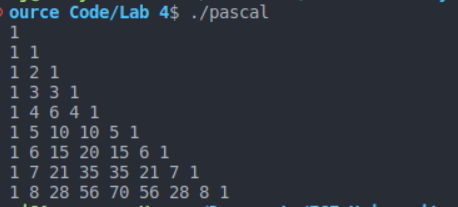
\includegraphics[width=15cm]{pascal.png}
		
\section{{Problem 2}}
	
		\subsection{{Computer Program}}
	
			\begin{lstlisting}[language=C, caption=\textit{Program to calculate the Gross Pay of a series of workers}]	
/*  Program to calculate the Gross Pay of a series of workers   */

#include <stdio.h>

int main()
{
    int employee_number, number_of_shifts, number_of_hrs, total_hrs,i;
    double wage_rate, gross_pay;
    FILE * in;
    in = fopen("L4_data.txt", "r");

    while(!feof(in)){
        fscanf(in, " %d %d %lf", &employee_number, &number_of_shifts, &wage_rate);
        i = 1;
        total_hrs = 0;
        while(i<= number_of_shifts){
            fscanf (in, "%d", &number_of_hrs);
            total_hrs = total_hrs + number_of_hrs;
            i++;
            }
            if (total_hrs <= 15){
                gross_pay = total_hrs * wage_rate;
                }
            else if (total_hrs >15 && total_hrs <= 25){
                gross_pay = (total_hrs * wage_rate * 1.05);
                }
            else if (total_hrs > 25){
                gross_pay = (total_hrs * wage_rate * 1.10);
                }
        printf("Employee Number     Total Hours        Gross Pay\n");
        printf("%8d%18d%20.2lf\n\n",employee_number,total_hrs,gross_pay);
    }
    
        fclose(in);
        return(0);
}

	\end{lstlisting}

		\subsection{{Program Output Screenshot}}
			
			{}
			
			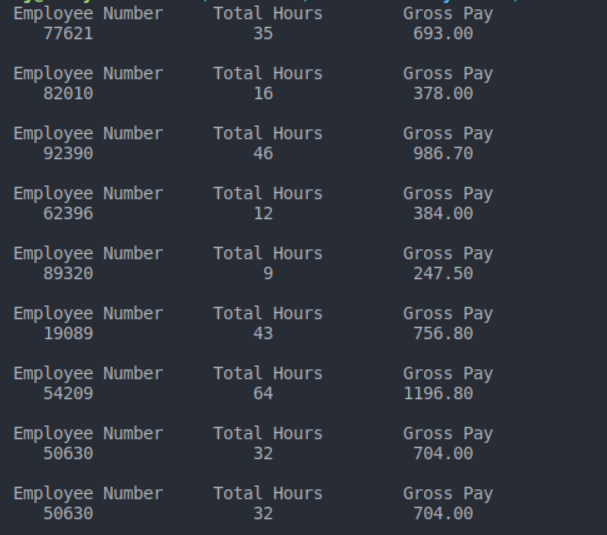
\includegraphics[width=12.75cm]{gross-pay.png}


\section{{Problem 3}}
	
	\subsection{{Computer Program}}
	
		\begin{lstlisting}[language=C, caption=\textit{Program to Calculate the Temperature-Pressure relation for some Temperature and Pressure}]	
/*  Program to Calculate the Temperature-Pressure relation for some Temperature and Pressure    */

#include <stdio.h>
#include <math.h>
#include <string.h>

float part_a(float initial_temperature, float initial_pressure, float final_pressure);
void part_b(float initial_temperature, float initial_pressure, float final_pressure, float max_temperature);

void main(void)
{
    float temp_i = 300;
    float pres_i = 50;
    float pres_f = 500;

    /*  Funtion to solve problem part a */
    float max_t = part_a(temp_i, pres_i, pres_f);

    /*  Funtion to solve problem part b */
    part_b(temp_i, pres_i, pres_f, max_t);
}

float part_a(float initial_temperature, float initial_pressure, float final_pressure)
{
    float max_temperature = (initial_temperature * final_pressure) / initial_pressure;
    printf("Maximum temperature the cylinder can withstand before bursting is %f\n", max_temperature);

    return max_temperature;
}

void part_b(float initial_temperature, float initial_pressure, float final_pressure, float max_temperature)
{
    int space = 4;

    /*  Header of the table */
    printf("Temperature (K)");
    for (int i = 0; i < space; i++)
    {
        printf(" ");
    }
    printf("Pressure (atm)\n");

    /*  Margins */
    for (int i = 0; i < strlen("Temperature (K)"); i++)
    {
        printf("-");
    }
    for (int i = 0; i < space; i++)
    {
        printf(" ");
    }
    for (int i = 0; i < strlen("Pressure (atm)"); i++)
    {
        printf("-");
    }
    printf("\n");    

    /*  Contents of the table*/
    for (float temperature = initial_temperature; temperature < max_temperature; temperature += 100)
    {
        /*  Calculating iterative pressure*/
        float pressure = (initial_pressure * temperature) / initial_temperature;

        /*  Calculating & tabulating the temperature-pressure relation  */
        printf("%.2f", temperature);
        for (int i = 0; i < strlen("Temperature (K)") - 5 + space; i++)
        {
            printf(" ");
        }
        printf("%.2f", pressure);
        for (int i = 0; i < strlen("Pressure (atm)") - 4; i++)
        {
            printf(" ");
        }

        /*  Line termination print  */
        printf("\n");
    }
}


	\end{lstlisting}
	
	\subsection{{Program Output Screenshot}}
	
		{}
		
		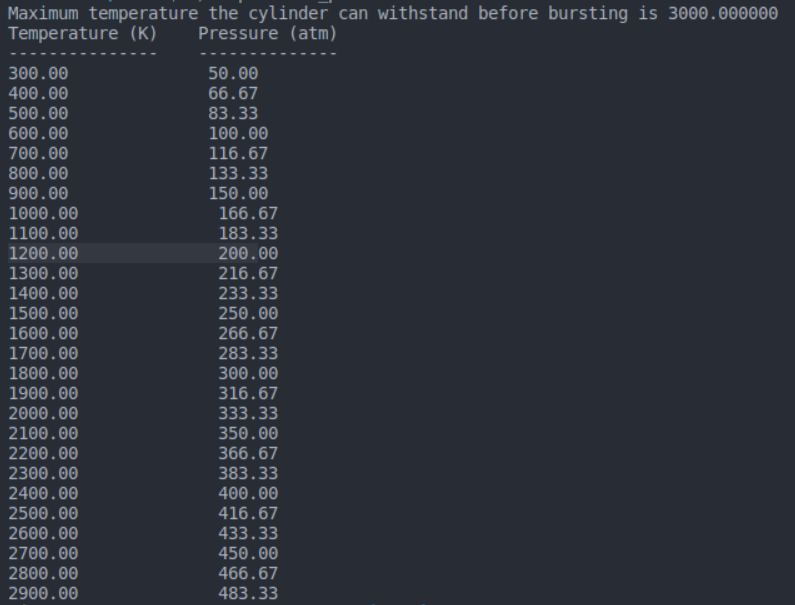
\includegraphics[width=12.75cm]{temp-pres.png}
		
		
		